\documentclass[UTF8]{ctexart}

\usepackage{geometry}
\geometry{a4paper, left=3cm, right=3cm, top=3cm, bottom=3cm}

%\usepackage{fontspec}
\usepackage{float}

\usepackage{graphicx}
\usepackage{svg}

\usepackage{minted}
%\usepackage{hyperref}
% \hypersetup{
%     colorlinks=true,
%     linkcolor=blue,
%     urlcolor=blue,
%     citecolor=blue
% }

\title{验证自动化流程设计说明}
\author{孙林涵,诸人豪,张煜}
\date{\today}

\begin{document}

%\maketitle
\begin{titlepage}
    \centering
    \vspace*{3cm}
    
    {\Huge \bfseries 华为杯\\[1em]
    第八届中国研究生创“芯”大赛\\[3em]}
    
    {\LARGE 验证自动化流程设计说明\\[5em]}
    
    {\Large
    作品名称:混沌逻辑-大模型多智能体自动数字IC前端设计器\hspace{6cm} \\[2em]
    团队名称:混沌逻辑\hspace{6cm} \\[2em]
    参赛队员:孙林涵,诸人豪,张煜\hspace{6cm} \\[5em]
    }
    
    \vfill
    {\large \today}
\end{titlepage}

\tableofcontents

\begin{abstract}
本软件通过设置项目管理、设计工程师和验证工程师三个Agent,模仿一般的IC设计流程,使通用大语言模型(LLM)生成可靠的RTL代码。本文档将详细介绍软件各个Agent的设计,以及软件的运行流程。
\end{abstract}

\newpage

\section{介绍}
%简要介绍文档背景和目的。
近年来,随着大语言模型(Large Language Model, LLM)技术逐渐进入应用场景,越来越多的领域开始尝试使用LLM来辅助工作。
数字前端设计作为一个复杂的工程领域,也开始探索如何利用LLM来提高设计效率和准确性。
然而,与其他领域相比,本领域的RTL代码开源少、且开源代码缺乏高质量设计;HDL语言与LLM大量学习的软件语言看似相似,实则在基础思路上存在着巨大差距。
此外,和LLM已取得广泛应用的软件工程相比,IC设计的容错率极低,对代码正确率要求高。
因此,直接调用已有的通用LLM到数字前端设计中是极不合理的。

为了解决这些问题,本项目设计了一套由通用LLM驱动的RTL代码的生成与验证自动化软件,旨在提高IC设计的效率和准确性。

\section{自动化系统设计}

本项目的设计目标是,在使用市场上现有的通用LLM的同时,最大化地减少LLM的幻觉,按照用户预期快速、自动地完成初版设计。
为此,我们仿照现有的IC设计流程设计了多个智能体(Agent),逐步展开用户的需求;并在LLM运行的各个阶段尽可能地使用Synopsys工具链对大模型的结果提出反馈,避免设计错误在工作流中传导。

\subsection{Agent设计}
考虑到前面提到的问题,期望LLM在单轮对话中直接给出正确的RTL设计是不现实的。
要确保大模型的输出正确且符合用户需求,则需要为LLM提供反馈,在多轮迭代后取得期望的输出。
但是,LLM的输出较慢(如本项目使用的Deepseek API仅能达到40~Token/s),若依赖人类产生反馈信息,则将占用用户大量时间,背离了自动化的设计初衷。
因此,本项目模仿一般的IC设计流程,设置了项目管理、设计工程师和验证工程师三个Agent,每个Agent均具有单独的短期记忆、长期记忆,并根据其职责设计了对应的工具供其使用。
LLM在使用工具时,间接调用了Synopsys的VCS等工具进行语法检查、仿真等,输出的结果将自动地反馈给大模型,实现了一定程度的自动化。
下面详细介绍各个Agent的设计。

\subsubsection{项目工程师Agent}
项目工程师解读用户输入的需求,生成项目的技术规范(下文简称Spec),并将其存储在文件中。
当设计完成时,项目工程师还会根据验证工程师的验证报告,检查设计是否满足规范要求。

\textbf{系统提示词:}
\inputminted[
  fontsize=\small,
  frame=lines,
  bgcolor=gray!10,
  breaklines=true
]{markdown}{../../prompt/proj_manager/system_prompt.md}

\textbf{用户提示词,根据用户输入生成完整spec时:}
\inputminted[
  fontsize=\small,
  frame=lines,
  bgcolor=gray!10,
  breaklines=true
]{markdown}{../../prompt/proj_manager/create_spec.md}

\textbf{用户提示词,验收项目时:}
\inputminted[
  fontsize=\small,
  frame=lines,
  bgcolor=gray!10,
  breaklines=true
]{markdown}{../../prompt/proj_manager/review_veri.md}

\textbf{工具:}
\begin{minted}[fontsize=\small, frame=lines, bgcolor=gray!10, breaklines=true]{python}
submit_spec = {
    "type": "function",
    "function": {
        "name": "submit_spec",
        "description": "提交SPEC文档。",
        "strict": True,
        "parameters": {
            "type": "object",
            "properties": {
                "spec": {"type": "string", "description": "SPEC文档内容"},
                "overwrite": {"type": "boolean", "description": "true表示覆盖现有的SPEC,false表示将其追加到现有SPEC中"}
            },
            "required": ["spec", "overwrite"],
            "additionalProperties": False
        }
    }
}
        
accept_report = {
    "type": "function",
    "function": {
        "name": "accept_report",
        "description": "批准当前报告。",
        "strict": True
    }
}

\end{minted}

\subsubsection{设计工程师Agent}
设计工程师根据项目工程师提供的Spec,生成RTL代码。设计工程师会将生成的代码存储在文件中,并在必要时进行修改。为避免LLM生成的代码存在语法错误,每次设计工程师提交代码时,都会使用VCS的vlogan工具进行语法检查。若检查出语法错误,设计工程师会根据错误信息进行修改,直到消除所有报错为止。

另外,设计工程师还会根据验证工程师的反馈,修改RTL代码以满足验证需求。

\textbf{系统提示词:}
\inputminted[
  fontsize=\small,
  frame=lines,
  bgcolor=gray!10,
  breaklines=true
]{markdown}{../../prompt/design_engineer/system_prompt.md}

\textbf{用户提示词,生成RTL代码时:}
\inputminted[
  fontsize=\small,
  frame=lines,
  bgcolor=gray!10,
  breaklines=true
]{markdown}{../../prompt/design_engineer/create_design.md}

\textbf{工具:}
\begin{minted}[fontsize=\small, frame=lines, bgcolor=gray!10, breaklines=true]{python}
submit_design = {
    "type": "function",
    "function": {
        "name": "submit_design",
        "description": "提交你的 Verilog 设计代码。设计代码将保存在一个 .v 文件中。你的设计代码在提交后会自动进行语法检查。",
        "strict": True,
        "parameters": {
            "type": "object",
            "properties": {
                "code": {"type": "string", "description": "Verilog设计代码"}
            },
            "required": ["code"],
            "additionalProperties": False
        }
    }
}
\end{minted}



\subsubsection{验证工程师Agent}
验证工程师根据项目工程师提供的Spec与用户提供的验证方案,生成验证计划,并编写测试用例。验证工程师会使用VCS编译仿真程序,并运行测试用例,生成验证报告。同样,当编译仿真程序时,若出现编译错误,验证工程师也会根据错误信息进行修改,直至成功编译得到simv仿真程序为止。
接下来,验证工程师会检查simv仿真程序的输出,判断RTL代码是否存在问题。当RTL代码存在问题时,验证工程师会将问题反馈给设计工程师,并要求其修改RTL代码。当验证工程师认为RTL代码满足验证需求时,会将验证报告提交给项目工程师。

\textbf{系统提示词:}
\inputminted[
  fontsize=\small,
  frame=lines,
  bgcolor=gray!10,
  breaklines=true
]{markdown}{../../prompt/veri_engineer/system_prompt.md}

\textbf{用户提示词,生成testbench时:}
\inputminted[
  fontsize=\small,
  frame=lines,
  bgcolor=gray!10,
  breaklines=true
]{markdown}{../../prompt/veri_engineer/create_tb.md}

\textbf{工具:}
\begin{minted}[fontsize=\small, frame=lines, bgcolor=gray!10, breaklines=true]{python}
submit_testbench = {
    "type": "function",
    "function": {
        "name": "submit_testbench",
        "description": "提交你的 Testbench 代码。Testbench 将保存在一个 tb.v 文件中",
        "strict": True,
        "parameters": {
            "type": "object",
            "properties": {
                "code": {"type": "string", "description": "Testbench代码"}
            },
            "required": ["code"],
            "additionalProperties": False
        }
    }
}
write_feedback = {
    "type": "function",
    "function": {
        "name": "write_feedback",
        "description": "撰写验证反馈。",
        "strict": True,
        "parameters": {
            "type": "object",
            "properties": {
                "text": {"type": "string", "description": "验证反馈"}
            },
            "required": ["text"],
            "additionalProperties": False
        }
    }
}
write_verification_report = {
    "type": "function",
    "function": {
        "name": "write_verification_report",
        "description": "撰写验证报告。",
        "strict": True,
        "parameters": {
            "type": "object",
            "properties": {
                "report": {"type": "string", "description": "验证报告"}
            },
            "required": ["report"],
            "additionalProperties": False
        }
    }
}
\end{minted}

\subsection{运行流程设计}
接下来,介绍本软件是如何调用各个Agent以完成RTL代码的生成与验证的。

图\ref{fig:flowchart}展示了本软件的运行流程。首先,项目工程师Agent会解读用户需求,生成Spec并存储在文件中。接着,设计工程师Agent会根据Spec生成RTL代码,并进行语法检查。若存在语法错误,设计工程师会进行修改。然后,验证工程师Agent会根据Spec与验证方案生成验证计划,并编写测试用例。验证工程师会编译仿真程序并运行测试用例,生成验证报告。当RTL代码存在问题时,验证工程师会将问题反馈给设计工程师,设计工程师会修改RTL代码并重新提交。最终,当验证工程师认为RTL代码满足验证需求时,会将验证报告提交给项目工程师。项目工程师确认RTL代码满足规范要求后,整个流程结束。

为了避免设计工程师的错误误导验证工程师,设计工程师和验证工程师将分别根据项目工程师提供的Spec与用户提供的验证方案生成各自的代码和测试用例。整个流程中多次出现的语法检查和编译步骤,确保了生成的代码和测试用例都是正确的。


%流程图
\begin{figure}[H]
    \centering
    \includesvg[width=0.99\textwidth]{flow.drawio.svg}
    \caption{程序流程图}
    \label{fig:flowchart}
\end{figure}




\section{运行过程展示与分析}
在本章中,我们展示本系统是如何协助我们完成赛题要求的设计的。
根据赛题要求,我们首先将需求的设计拆分成多个模块,其结构如图~\ref{fig:hardsch}所示。
经我们考虑,此步骤过于复杂,不可能交由LLM实现,因此此部分由人工进行。

%框图
\begin{figure}[H]
    \centering
    \includesvg[width=0.99\textwidth]{../1-完整设计规范说明书/schematic.svg}
    \caption{硬件框图}
    \label{fig:hardsch}
\end{figure}

在拆分子模块后,我们将使用自然语言描述各个模块的IO信号、功能等,并设计验证时的参考模型。
下面以fifo\_data\_resolu为例子,介绍本系统的运行情况。

requirements.md 中描述了用户对该模块的需求,如下所示。

\textbf{challenge/module3/requirements.md}
\inputminted[
  fontsize=\small,
  frame=lines,
  bgcolor=gray!10,
  breaklines=true
]{markdown}{../../challenge/module3/requirements.md}

veri\_plan.md 中简要提出了用户对验证的要求,如下所示。

\textbf{challenge/module3/veri\_plan.md}
\inputminted[
  fontsize=\small,
  frame=lines,
  bgcolor=gray!10,
  breaklines=true
]{markdown}{../../challenge/module3/veri_plan.md}

为了确保设计符合预期,我们还为系统提供了参考模型,如下所示。

\textbf{challenge/module3/ref\_model/ref\_model.sv}
\inputminted[
  fontsize=\small,
  frame=lines,
  bgcolor=gray!10,
  breaklines=true
]{verilog}{../../challenge/module3/ref_model/ref_model.sv}


项目管理员首先根据输入生成了完整的Spec:

\textbf{fifo\_data\_resolu/spec.md}
\inputminted[
  fontsize=\small,
  frame=lines,
  bgcolor=gray!10,
  breaklines=true
]{markdown}{./spec.md}

根据完整的Spec,设计工程师进行了多轮迭代,其详细过程过长,在提交文档中的‘3-LLM运行’文件夹中给出。在几次迭代后,成功的设计如下:

\textbf{fifo\_data\_resolu/design/dut.v}
\inputminted[
  fontsize=\small,
  frame=lines,
  bgcolor=gray!10,
  breaklines=true
]{verilog}{./dut.v}

同上,验证工程师的迭代过程也不再此处赘述。
根据完整的Spec和用户生成的参考模型,验证工程师提供的最终Testbench如下:

\textbf{fifo\_data\_resolu/verification/tb.sv}
\inputminted[
  fontsize=\small,
  frame=lines,
  bgcolor=gray!10,
  breaklines=true
]{verilog}{./tb.sv}

运行该Testbench,可以看到全部设计通过,覆盖率如图~\ref{fig:cov}所示。

\begin{figure}[H]
    \centering
    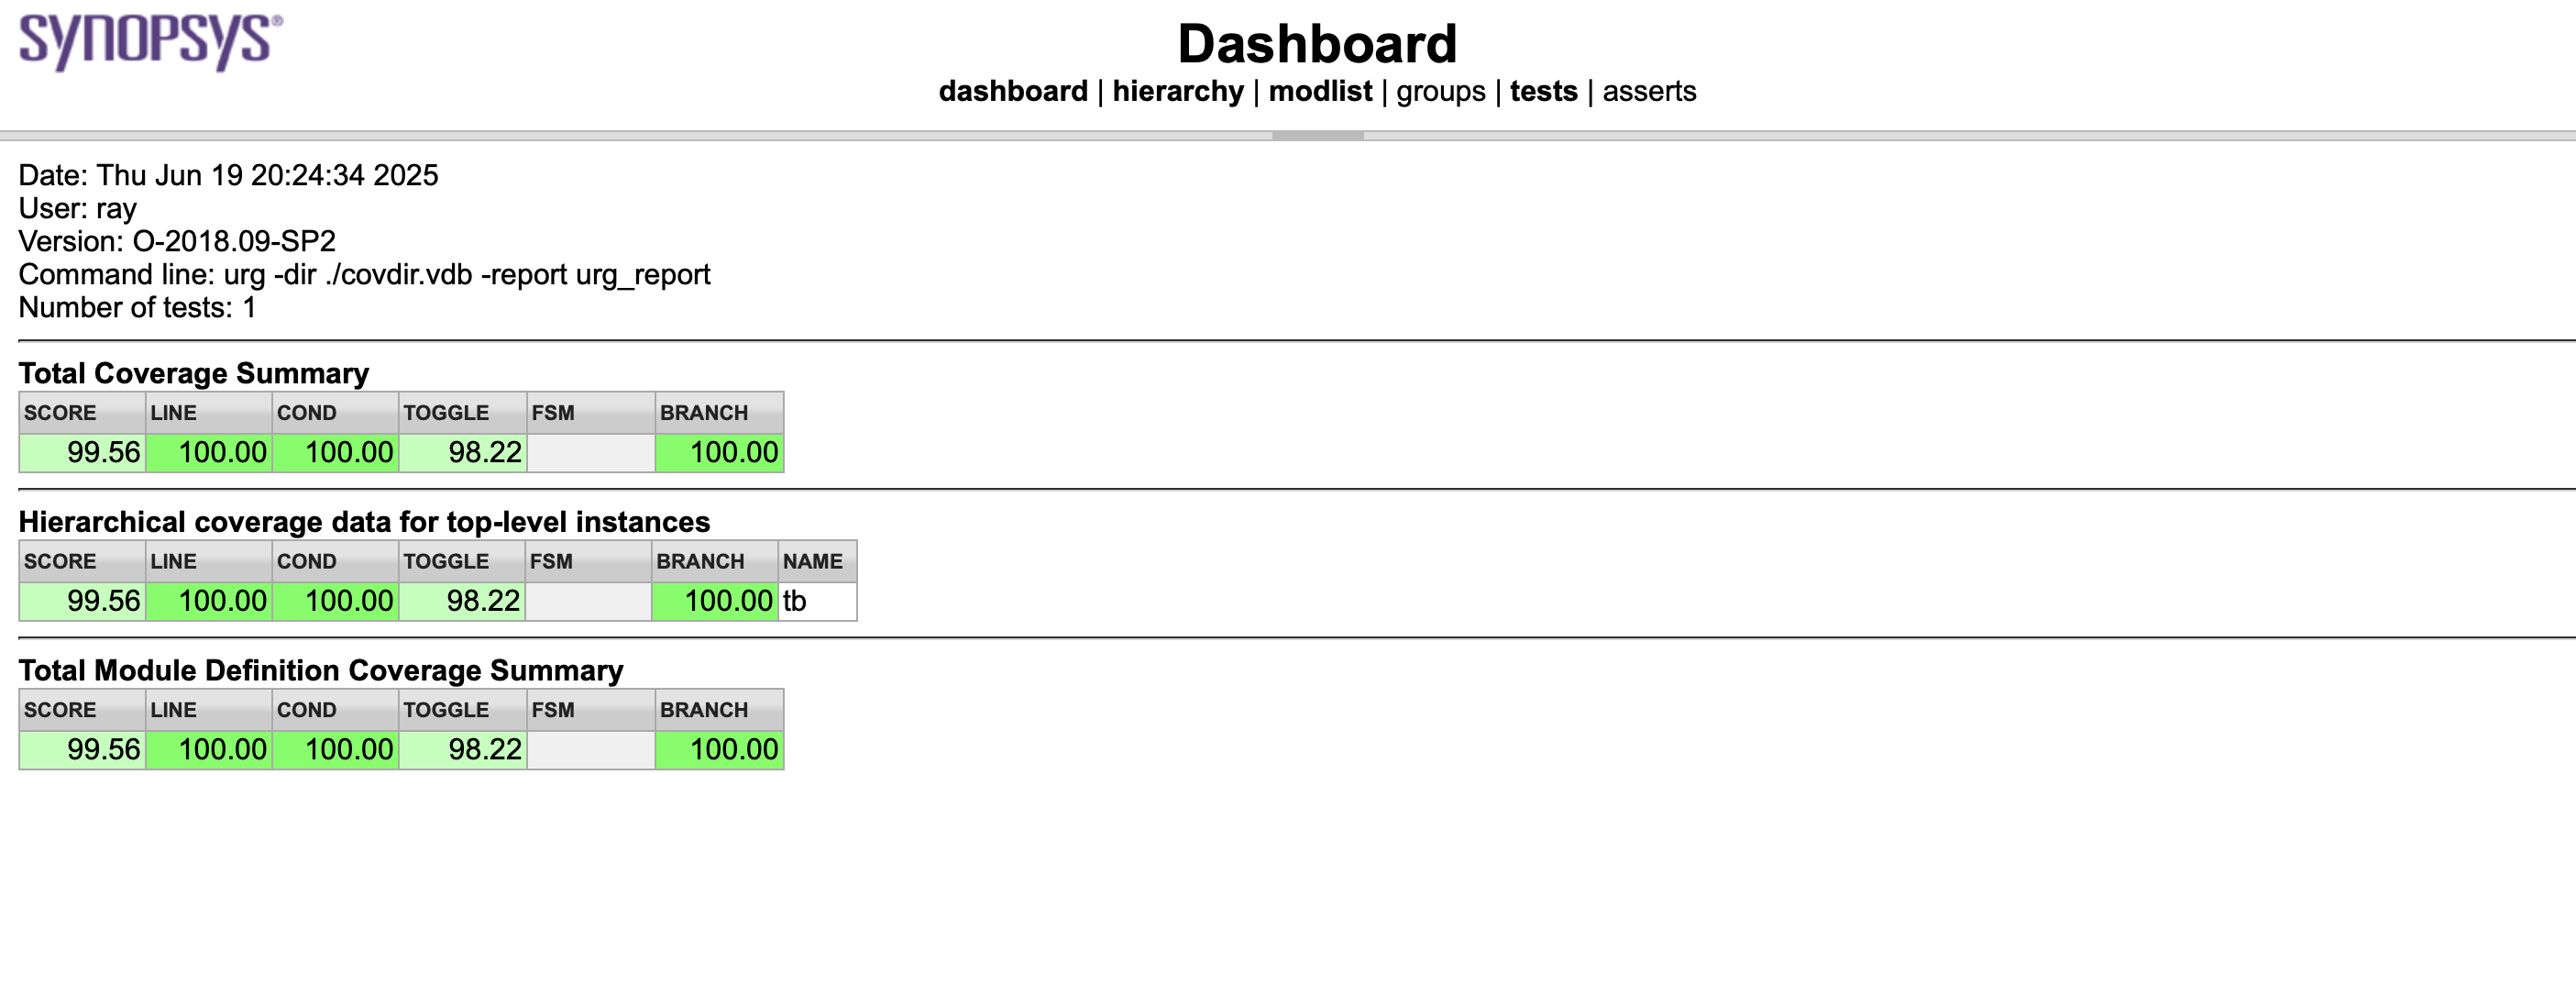
\includegraphics[width = 0.90\textwidth]{cov.png}
    \caption{覆盖率}
    \label{fig:cov}
\end{figure}

可以看到,LLM设计的Testbench成功覆盖了本模块的绝大部分内容,整体的代码覆盖率达到了99.56\%。

验证工程师Agent根据验证结果,提交了对应的验证报告:

\textbf{verification\_report.md}
\inputminted[
  fontsize=\small,
  frame=lines,
  bgcolor=gray!10,
  breaklines=true
]{markdown}{../7-验证报告/fifo_data_resolu/verification_report.md}

\section{总结}
本项目设计了一套由LLM驱动的RTL代码的生成与验证自动化软件,实现了IC设计流程的自动化,能够快速产出原型设计。然而,在设计中,我们发现,一般的通用大模型在数字电路相关任务上、尤其是验证任务上,存在相当大的局限性。要进一步减少本项目的迭代次数,提升设计效率,必须对大模型进行针对性的训练,以使其能够更好地理解数字电路的设计与验证流程。本项目产出的原型设计,也应由专业的设计工程师和验证工程师进行进一步的修改与验证,以确保其满足实际的设计需求。

\end{document}